%%%%%%%%%%%%%%%%%%%%%%%%%%%%
%%%%%%%%% IMPORTS %%%%%%%%%%
%%%%%%%%%%%%%%%%%%%%%%%%%%%%
\documentclass[a4paper,12pt]{article}

\usepackage{comment}
\usepackage{supertabular}
\usepackage{graphics}
\usepackage{color,soul}
\usepackage{booktabs}
\usepackage{paralist}
\usepackage{algorithmicx}
\usepackage{algorithm}
\usepackage[noend]{algpseudocode}
\usepackage{booktabs}
\usepackage{hvfloat}
\usepackage{comment}
\usepackage{chngpage}
\usepackage{url}
\usepackage[utf8]{inputenc}
\usepackage[table,dvipsnames]{xcolor}
\usepackage[a4paper,pdftex,hmargin=0.75in,vmargin={1.1in,0.6in},head=75pt,foot=45pt, left=2.5cm, right=2.5cm, includefoot, footskip=60pt]{geometry}
\usepackage{lipsum}
\usepackage{afterpage}
\usepackage{xcolor}
\usepackage{tabularx}
\usepackage{wallpaper}
\usepackage{adjustbox}
\usepackage[normalem]{ulem}
\useunder{\uline}{\ul}{}
\usepackage{rotating}
\usepackage{parskip}
\usepackage{listings}
\lstset{language=C,breaklines=true}
\usepackage[english]{babel}
\usepackage{amsmath}
\usepackage{amsfonts}
\usepackage{amssymb}
\usepackage[justification=centering]{caption}
\usepackage{fontenc}
\usepackage{multicol}
\usepackage{multirow}
\usepackage{array}
\usepackage{relsize}
\usepackage{subcaption}
\usepackage{caption}
\usepackage[colorlinks=true,pdfusetitle]{hyperref}
\usepackage{tcolorbox}
\usepackage{lscape}
\usepackage{lastpage}
\usepackage{acro}
\setlength{\headsep}{1.5cm}
\usepackage[toc,page]{appendix}
\usepackage[nottoc]{tocbibind} % for show references in toc
\usepackage{pgfgantt}
\frenchspacing
%\usepackage{svg}
%\usepackage{showframe}% for show page layout

%%%%%%%%%%%%%%
% Set by Oscar
%%%%%%%%%%%%%%
\usepackage{microtype}
\usepackage[newfloat,draft=false]{minted}

\colorlet{punct}{red!60!black}
\definecolor{background}{HTML}{EEEEEE}
\definecolor{delim}{RGB}{20,105,176}
\colorlet{numb}{magenta!60!black}
\lstdefinelanguage{json}{
    basicstyle=\normalfont\ttfamily,
    numbers=left,
    numberstyle=\scriptsize,
    stepnumber=1,
    numbersep=8pt,
    showstringspaces=false,
    breaklines=true,
    frame=lines,
    backgroundcolor=\color{background},
    literate=
     *{0}{{{\color{numb}0}}}{1}
      {1}{{{\color{numb}1}}}{1}
      {2}{{{\color{numb}2}}}{1}
      {3}{{{\color{numb}3}}}{1}
      {4}{{{\color{numb}4}}}{1}
      {5}{{{\color{numb}5}}}{1}
      {6}{{{\color{numb}6}}}{1}
      {7}{{{\color{numb}7}}}{1}
      {8}{{{\color{numb}8}}}{1}
      {9}{{{\color{numb}9}}}{1}
      {:}{{{\color{punct}{:}}}}{1}
      {,}{{{\color{punct}{,}}}}{1}
      {\{}{{{\color{delim}{\{}}}}{1}
      {\}}{{{\color{delim}{\}}}}}{1}
      {[}{{{\color{delim}{[}}}}{1}
      {]}{{{\color{delim}{]}}}}{1},
}

%RBG FFD33E / C95D40
\definecolor{upcorange}{HTML}{FFD33E}
\hypersetup{linkcolor=blue}

% probably a good idea for the nomenclature entries:
\acsetup{first-style=short}

%%%% PAGE STYLE %%%%%
\usepackage{fancyhdr}
\pagestyle{fancy}
\fancyhf{}
\lhead{
\includegraphics[height=1.2cm]{img/logos/upclogo.png}}
\rhead{
\includegraphics[height=1.2cm]{img/logos/logo_telecos.png}}
\rfoot{\thepage{}}

\renewcommand{\footrulewidth}{0.4pt}
%\futurelet\TMPfootrule\def\footrule{{\color{upcorange}\TMPfootrule}}
\futurelet\TMPfootrule\def\footrule{{\color{gray!80}\TMPfootrule}}
\renewcommand{\headrulewidth}{0.4pt}
\renewcommand{\headrule}{\hbox to\headwidth{%
%\color{upcorange}\leaders\hrule height \headrulewidth\hfill}}
\color{gray!80}\leaders\hrule height \headrulewidth\hfill}}
%\renewcommand*\ShowFrameColor{\color{red}}

%%% TEMPORAL
%% for 1.5 line spacing
\usepackage{setspace}
\onehalfspacing

%% TODO command
\newcommand{\TODO}[1]{ 
\begin{tcolorbox}[colback=red!5!white,colframe=red!75!black]
  TODO: #1

  date: \today
\end{tcolorbox}
}


%%%%%%%%%%%%%%%%%%%%%%%%%%%%%%%%%%%
%% DOCUMENT: main.tex            %%
%% AUTHOR: Òscar Pérez Castillo  %%
%% UNIVERSITY: UPC               %%
%% DATE: 02/06/2021              %%
%% VERSION: v0.1                 %%
%%%%%%%%%%%%%%%%%%%%%%%%%%%%%%%%%%%
\title{Development of a LXD framework}
\author{Òscar Pérez Castillo}

\begin{document}

%%% COVER %%%
\fancypagestyle{alim}{\fancyhf{}\renewcommand{\headrulewidth}{0pt}
    \cfoot{
\includegraphics[height=2.2cm]{img/logos/logo_telecos.png}}
}
\thispagestyle{empty}
\begin{center}
    {\sffamily
        \resizebox{0.8\textwidth}{!}{
\includegraphics{img/logos/upc_completo+telecos.png}}\\
        \vspace{1cm}
        {\Huge Thesis title}\\
        \vspace{0.5cm}
        {\color{black}\hrule height 1pt}
        \vspace{1cm}
        {\large{Oscar Perez Castillo Thesis / Treball Fi de Grau / Trabajo Fin de Grado\\
                submitted to the Faculty of the / realitzada a l' / realizada en la \\
                Escola T\`ecnica d'Enginyeria de Telecomunicaci\'o de Barcelona \\
                Universitat Polit\`ecnica de Catalunya \\
                by / per / por \\
                \vspace{0.5cm}
                %{\Huge{Student name}}
                Student name}}

        \vspace{1.5cm}

        {In partial fulfillment / En compliment parcial / En cumplimiento parcial\\
            of the requirements for the degree in / dels requisits per al Grau en / de los requisitos para el Grado en \\
            \textit{(Write the name of your Degree)} \textbf{ENGINEERING}}

        \vspace{2cm}

        {{Advisor / Director/ Directora: name of the advisor\\}}
        {{Barcelona, Date XXXXX}}

        \vspace{2cm}

        {\color{red} \textbf{Note:} Please note this frontpage is provided in the three official languages. Please select one and delete this note as well.}
        \thispagestyle{alim}
    }

\end{center}


%%%%%%%%%%%%%%%%%%%%%%%%%%%%%%%%%%%%%%
%%% ABSTRACT AND REVISION HISTORY %%%%
%%%%%%%%%%%%%%%%%%%%%%%%%%%%%%%%%%%%%%

%%% ABSTRACT %%%
\newpage
\section*{Abstract}
 {Every copy of the thesis the thesis must have an abstract. An abstract must provide a concise summary of the thesis. In style, the
  abstract should be a miniature version of the thesis: short introduction, a summary of the results, conclusions or main
  arguments presented in the thesis. The abstract may not exceed 150 words for a Degree’s thesis.
  Pruebas:
  \cite{einstein}
  \ref{sec:introduction}
  }

\addcontentsline{toc}{section}{Abstract}

\newpage
\section*{Revision history and approval record}
\begin{center}
\tablefirsthead{}
\tablehead{}
\tabletail{}
\tablelasttail{}
\begin{supertabular}{|m{1.908cm}|m{2.398cm}|m{11.489cm}|}
\hline
\selectlanguage{english} \foreignlanguage{english}{\textbf{Revision}} &
\selectlanguage{english} \foreignlanguage{english}{\textbf{Date}} &
\selectlanguage{english} \foreignlanguage{english}{\textbf{Purpose}}\\\hline
\selectlanguage{english} \foreignlanguage{english}{0} &
\selectlanguage{english} \foreignlanguage{english}{01/06/2021} &
\selectlanguage{english} \foreignlanguage{english}{Document \ creation}\\\hline
\selectlanguage{english} \foreignlanguage{english}{1} &
\selectlanguage{english} \foreignlanguage{english}{dd/mm/yyyy} &
\selectlanguage{english} \foreignlanguage{english}{Document \ revision}\\\hline
~
 &
~
 &
~
\\\hline
~
 &
~
 &
~
\\\hline
~
 &
~
 &
~
\\\hline
\end{supertabular}
\end{center}

\bigskip

\selectlanguage{english}
DOCUMENT DISTRIBUTION LIST

\begin{center}
\tablefirsthead{}
\tablehead{}
\tabletail{}
\tablelasttail{}
\begin{supertabular}{|m{8.205cm}|m{7.589cm}|}
\hline
\selectlanguage{english} \foreignlanguage{english}{\textbf{\ Name}} &
\selectlanguage{english} \foreignlanguage{english}{\textbf{\ e-mail}}\\\hline
\selectlanguage{english} \foreignlanguage{english}{Òscar Pérez Castillo} &
~ \href{mailto:oscar.pz.castillo@gmail.com}{oscar.pz.castillo@gmail.com}
\\\hline
\selectlanguage{english} \foreignlanguage{english}{Jose Luis Muñoz Tapia} &
~
\\\hline
\selectlanguage{english} \foreignlanguage{english}{Rafael Genés Duran} &
~
\\\hline
~
 &
~
\\\hline
~
 &
~
\\\hline
~
 &
~
\\\hline
\end{supertabular}
\end{center}

\bigskip

\begin{center}
\tablefirsthead{}
\tablehead{}
\tabletail{}
\tablelasttail{}
\begin{supertabular}{|m{1.925cm}|m{6.1990004cm}|m{1.901cm}|m{5.6140003cm}|}
\hline
\multicolumn{2}{|m{8.324cm}|}{ Written by:} &
\multicolumn{2}{m{7.715cm}|}{Reviewed and approved by:}\\
\hline
\selectlanguage{english} Date &
\selectlanguage{english} dd/mm/yyyy &
\selectlanguage{english} Date &
\selectlanguage{english} dd/mm/yyyy\\\hline
\selectlanguage{english} Name &
\selectlanguage{english} Xxxxxxx yyyyyyy &
\selectlanguage{english} Name &
\selectlanguage{english} \foreignlanguage{english}{Zzzzzzz \ Wwwwwww}\\\hline
\selectlanguage{english} Position &
\selectlanguage{english} \foreignlanguage{english}{Project Author } &
\selectlanguage{english} \foreignlanguage{english}{Position} &
\selectlanguage{english} \foreignlanguage{english}{Project Supervisor}\\\hline
\end{supertabular}
\end{center}

\addcontentsline{toc}{section}{Revision history}


%%% INDEX %%%
\newpage
\tableofcontents

\addcontentsline{toc}{section}{Contents}

\newpage
\listoffigures

\newpage
\lstlistoflistings
\addcontentsline{toc}{section}{Listings}




%%%%%%%%%%%%%%%%%%%%%%%%%%%%%%
%%% INTRODUCTION: SECTIONS %%%
%%%%%%%%%%%%%%%%%%%%%%%%%%%%%%

%%% 01-INTRODUCTION %%%
\newpage
%%%%%%%%%%%%%%%%%%%%%
%% 01-INTRODUCTION %%
%%%%%%%%%%%%%%%%%%%%%
\clearpage\section{Introduction}

%%% Introduction %%%
Virtualization is a computer mechanism that allows a single computer to host multiple virtual machines, where each system has the ability of running a completely different operating system than the main machine. 

One kind of virtualization it is the 'OS-level virtualization' (or containerization), which is a paradigm in which the operating system, throught different os level functionalities, can create user instances, where those instances are what we refer as "containers" as they have their own set of os-resources properties in their own environment.

On top of that technology, several systems and technologies have emerged over the years. In Linux, the "Linux Containers project" has been working on containers for over ten years and has develop a set of utilities to provide a framework as close as what you get from a VM (virtual machine). 

One of that utilities is 'LXC/LXD'. These utilities are a set of tools that allow us to run unmodified Linux distributions inside containers without the overhead of creating a virtual machine. This is extremely helpfull because we can create diferent linux distributions in one unique linux machine.

So, the objective of this thesis is to provide a framework on top of the 'LXC/LXD' utilities to unify some of their commands and improve the management of the containers.

\bigskip

%%% SECTION: Requirement and specifications %%%
\subsection{Requirements and specifications}
\label{ssec:requirements}
The "lxc/lxd" set of tools are used for creating such "containers". Once created, we can start/stop them, add them shared folders, manage memory, manage cpu resources, set up linux distribution ...
But a lot of commands for properly set up a container with diferents configurations (folders, proxies...) were needed. Also, when the number of containers increase, we have no way or organize them of categorize them.

So the requirements, based on those problems, were:
\begin{itemize}
	\item {Be able to manage a common container configuration by a text file}
	\item {Possibiliy to group containers by "domains"}
	\item {Tag containers by an alias name}
	\item {Set up proxies based on a text file}
\end{itemize}

By developing the following base of tools:
\begin{itemize}
	\item {\textbf{lxce}: base command installed on top of "lxc". Should be responsible for configuring all the containers based on configuration files and commands.}
	\item {\textbf{lxce-admin}: command for managing the different hosts with lxce installed in a centralized location}
	\item {\textbf{web interface}: minimal web application for visualiazing all the containers and manage them with a simple API}
\end{itemize}


%%% SECTION: Previous efforts %%%
\subsection{Previous efforts}
\label{ssec:previous}
The thesis began with the two commands (lxce and lxce-admin) in an initial version:
\begin{itemize}
	\item {\textbf{lxce}: this command was in an initial version but it lack a lot of different features along robusteness}
	\item {\textbf{lxce-admin}: this command was simple but should be extended for improve some features}
\end{itemize}
The two were written in Javascript.

For the web interface no versions were made, so it should be coded from the beginning.

%%% SECTION: Work plan %%%
\subsection{Work plan}
\label{ssec:gantt}
For the work plan we set the following goals, in order of preference:
\begin{itemize}
	\item {Develop a robust, well tested version for the "lxce" command}
	\item {Integrated the improvements in the centralized "lxce-admin" command}
	\item {Based on left time, develop the web interface application}
\end{itemize}

\newpage
Where we can see summaritze it in:
\begin{figure}[H]
    \begin{ganttchart}[y unit title=0.4cm,
y unit chart=0.5cm,
vgrid,hgrid,
title height=1,
%today=25,%
%today offset=.5,%
%today label=Now,%
%bar/.style={draw,fill=cyan},
bar incomplete/.append style={fill=yellow!50},
bar height=0.7]{1}{24}

 % dies
 \gantttitle{Phases of the Project}{24} \\
 \gantttitle{2021}{24} \\
 \gantttitle{Feb}{4}
 \gantttitle{Mar}{5}
 \gantttitle{April}{5}
 \gantttitle{May}{5}
 \gantttitle{Jun}{5} \\
 
 % caixes elem0 .. elem9 
 % INTRODUCTION
 \ganttgroup[inline=false]{Introduction}{1}{2}\\
 \ganttbar[progress=100,bar/.style={draw,fill=cyan}]{Learn Javascript}{1}{1} \\
 \ganttbar[progress=100,bar/.style={draw,fill=cyan}]{Learn about containers}{2}{2} \\

 % LXCE
 \ganttgroup[inline=false]{lxce}{3}{16}\\
 \ganttbar[progress=100,bar/.style={draw,fill=red}]{v0.1}{3}{5} \\
 \ganttbar[progress=100,bar/.style={draw,fill=red}]{v0.2}{6}{8} \\
 \ganttbar[progress=100,bar/.style={draw,fill=red}]{v0.3}{9}{16} \\

 % LXCE-ADMIN
 \ganttgroup[inline=false]{lxce-admin}{14}{16}\\
 \ganttbar[progress=100,bar/.style={draw,fill=white}]{v0.1}{14}{16} \\

 % WEB ADMIN
 \ganttgroup[inline=false]{lxce-admin}{17}{20}\\
 \ganttbar[progress=90,bar/.style={draw,fill=black}]{Learn React/redux}{17}{19} \\
 \ganttbar[progress=10,bar/.style={draw,fill=black}]{Implement application}{20}{20} \\

 % relations
\ganttlink{elem2}{elem4}
\ganttlink{elem8}{elem10}


\end{ganttchart}

    \caption[Project's Gantt diagram]{\footnotesize{Gantt diagram of the project}}
    \label{fig:gantt}
\end{figure}
where no significant incidences nor deviations ocurred.
\bigskip



%%% 02-STATE OF THE ART %%%
\label{sec:state}
\clearpage\section{State of the art of the technology used or applied in this thesis:}

 {A backgroundadajdasajdaskdasdsadsa, comprehensive review of the literature is required. This is known as the Review of Literature and should
  include relevant, recent research that has been done on the subject matter.}

\subsection{Topic}

Here you have a couple of references about LaTeX ~\cite{latexcompanion} and electrodynamics \cite{einstein}.

\bigskip

\subsection{Topic}


%%%%%%%%%%%%%%%%%%%%%%%%%%%%%%
%%% RESULTS: SECTIONS %%%%%%%%
%%%%%%%%%%%%%%%%%%%%%%%%%%%%%%

%%% 03-METHODOLY %%%
\clearpage
\label{sec:methodology}
%%%%%%%%%%%%%%%%%%%%
%% 03-METHODOLOGY %%
%%%%%%%%%%%%%%%%%%%%
\clearpage\section{Methodology / project development}

In order to construct our framework we had to develop a set of tools. Basically we developed two commands and a minimal web application:
\begin{itemize}
	\item{LXCE: command constructed on top of LXD}
	\item{LXCE-admin: }
	\item{Web-admin} 
\end{itemize}
\DUDA{explicar cada uno más detallado?? / los nombres de las herramientas en mayus o minus}

This chapter will provide with the technical implementation of each tool and how they are constructed and organized. 

%%% LXCE %%%
\subsection{LXCE}
The first tool developed in this thesis is what we have called 'lxce'.

It is basically a command line tool coded in Typescript built on top of the 'lxc' command line tool with the idea of improving the management and set up of the containers.
[TODO: site chapter]
\TODO{Site chapter}

The problem with the 'lxc' tool is that in order to have a properly set up container we would have to do the following steps, for every container:
\begin{itemize}
	\item{Create the container with linux image specified}
		\begin{minted}[bgcolor=background]{text}
host# lxc launch ubuntu:20.04 container
		\end{minted}
	\item{Configure password}
		\begin{minted}[breaklines,bgcolor=background]{text}
host# lxc exec ${name} -- bash -c "echo ${user}:${password} | chpasswd"
		\end{minted}
	\item{Set up shared folders}
		\begin{minted}[breaklines,bgcolor=background]{text}
host# lxc config device add containers myfolder disk source=/www/data path=/data
		\end{minted}
	\item{Set up proxies, selecting each time a non used host port}
		\begin{minted}[breaklines,bgcolor=background]{text}
host# lxc config device add myproxy proxy listen=tcp:0.0.0.0:4000 connect=tcp:10.1.2.1:80
		\end{minted}
\end{itemize}

Then, if we would like to access the containers by ssh or vnc we would have to create also the corresponding configuration files.

Everything is managed individually, which is good for a basic set up, but for situations where we are working with +50 containers is unmanagible??. 

So the idea of this command is to resolve such limitations with a command which could:
\begin{itemize}
	\item{Manage containers by configuration files, with a default configuration file}
	\item{Organize containers by "domains"}
	\item{Be able to reference containers by aliases}
	\item{Configure proxies and shared locations with a configuration file}
	\item{Generate SSH and VNC configuration files to be distributed}
\end{itemize}

Once defined all the specifications for the command we will explain how are the configuration files organized and the list of subcommands implemented.

\subsubsection{Configuration files}
The first thing we have to define are the configurations files and how are they are going to be organized.
\TODO{explain their usage in a general overview}

Firt of all, we will have 5 different types of configuration files:
\begin{itemize}
	\item{\textbf{container-default.conf}: default configuration file}
	\item{\textbf{lxce.conf}: general command configuration}
	\item{individual container configuration files}
	\item{\textbf{remmina} (vnc service) configuration files}
	\item{\textbf{ssh} configurations files}
\end{itemize}

So a basic set up with two domains (default and derecho) and one container created in each of the domains would look like:

\begin{listing}[H]
\begin{minted}[bgcolor=background]{text}
/etc/lxce 
|--- container.conf.d 			
|   |--- default 			
|   |   '--- voiceless-blue
|   '--- derecho 			
|       '--- relieved-beige
|--- container_default.conf 		
|--- lxce.conf 			
|--- remmina 		
|   |--- default 
|   |   '--- oscar-vm.default.voiceless-blue.remmina
|   '--- derecho 
|       '--- oscar-vm.derecho.relieved-beige.remmina
'--- ssh 	
    |--- default 
    |   '--- voiceless-blue.conf
    '--- derecho
        '--- relieved-beige.conf
\end{minted}
\caption{lxce directory structure}
\label{listings: lxce directory structure /etc/lxce}
\end{listing}

In this way we are able to manage the container configurations from our command line and update/delete files based on the state of the command.

Where the configurations files content is the following:
\begin{itemize}
%%%%%%%%%%
%% ITEM %%
%%%%%%%%%%
\newpage
\item{\textbf{container-default.conf}

This file acts as a template for every container to be created.
\begin{listing}[H]
\begin{minted}[bgcolor=background]{json}
{
  "name": "",                           
  "alias": "",                          
  "user": "",
  "id_domain": 0,
  "id_container": 0,

  "domain": "default",                 
  "base": "ubuntu:20.04",             
  "userData": "/datasdd",            

  "proxies": [                      
    {
      "name": "ssh",
      "type": "tcp",
      "listen": "0.0.0.0",
      "port": 22
    },
    {
      "name": "test",
      "type": "tcp",
      "listen": "0.0.0.0",
      "port": 3000
    }
  ],
}
\end{minted}
\caption{/etc/lxce/container-default.conf}
\label{listings: /etc/lxce/container-default.conf}
\end{listing}
\TODO{Think the convention for the name of the figures and the descriptions of the listings}
}
%%%%%%%%%%
%% ITEM %%
%%%%%%%%%%
\newpage
\item{\textbf{lxce.conf}

This file specifies different parameters of the host where the command is installed, such as:
\begin{itemize}
	\item{SSH IP}
	\item{Hostname}
	\item{Local VNC server configuration}
	\item{Seed used for generating passwords}
	\item{List of container domains currently in the host}
	\item{List of locations available for the shared containers folders location}
\end{itemize}
\begin{listing}[H]
\begin{minted}[bgcolor=background]{json}
{
  "hypervisor": {
    "SSH_hostname": "localhost",
    "SSH_suffix": "oscar-vm",
    "VNC_server": "localhost",
    "VNC_port": 5901
  },
  "seed": "4b5a003f0e1715df",
  "domains": [
    {
      "id": 0,
      "name": "default"
    },
    {
      "id": 1,
      "name": "derecho"
    }
  ],
  "locations": [
    "/datasdd"
  ]
}
\end{minted}
\caption{lxce.conf}
\label{listings: /etc/lxce/lxce.conf}
\TODO{explain all the parameters}
\end{listing}
}
%%%%%%%%%%
%% ITEM %%
%%%%%%%%%%
\newpage
\item{\textbf{container configuration file}

This files list the configured parameters for each container and the ids that uniquelly identifies it
\begin{listing}[H]
\begin{minted}[bgcolor=background]{json}
{
  "name": "voiceless-blue",
  "alias": "",
  "user": "ubuntu",
  "id_domain": 0,
  "id_container": 0,
  "domain": "default",
  "base": "ubuntu:20.04",
  "userData": "/datasdd",
  "proxies": [
    {
      "name": "ssh",
      "type": "tcp",
      "listen": "0.0.0.0",
      "port": 22
    },
    {
      "name": "test",
      "type": "tcp",
      "listen": "0.0.0.0",
      "port": 3000
    }
  ],
}
\end{minted}
\caption{container configuration file}
\label{listings: /etc/lxce/container.conf.d/default/voiceless-blue}
\end{listing}
}
%%%%%%%%%%
%% ITEM %%
%%%%%%%%%%
\clearpage
\item{\textbf{VNC configuration}
\begin{listing}[H]
\begin{minted}[bgcolor=background]{text}
[remmina]
ssh_tunnel_privatekey=
name=oscar-vm.default.voiceless-blue          # Container name
ssh_tunnel_passphrase=
password=.                                    # For saving VNC password
...
server=localhost:5901                         # VNC server
disablepasswordstoring=0
ssh_tunnel_username=ubuntu
disableclipboard=0
window_maximize=1
ssh_tunnel_password=.                         # For saving ssh password
enable-autostart=0
proxy=
ssh_tunnel_server=localhost:10000             # Container SSH Port
ssh_tunnel_auth=0
group=oscar-vm.upc.edu                        
...
protocol=VNC
username=ubuntu                               # VNC username
showcursor=0
colordepth=32

\end{minted}
\caption{REMMINA configuration file}
\label{listing: /etc/lxce/remmina/default/oscar-vm.default.voiceless-blue.remmina}
\end{listing}
}
%%%%%%%%%%
%% ITEM %%
%%%%%%%%%%
\item{\textbf{SSH configuration}
\begin{listing}[H]
\begin{minted}[bgcolor=background]{text}
Host oscar-vm.default.voiceless-blue
   Hostname localhost
   User ubuntu
   Port 10000
   TCPKeepAlive yes
   ServerAliveInterval 300
\end{minted}
\caption{ssh configuration file}
\label{listings: /etc/lxce/ssh/default/voiceless-blue.conf}
\end{listing}
}
\end{itemize}

\newpage
\subsubsection{Commands}
\DUDA{Explicar aqui como esta implementado??}
For the commands that are available for our command, we have the following structure:
\begin{minted}[bgcolor=background]{text}
Usage: lxce [command] <options> <flags>

Commands:
  lxce alias       Manage containers aliases
  lxce completion  Output completions scripts
  lxce delete      Delete containers and configurations/folders related
  lxce init        Initialize lxce command
  lxce launch      Launch containers
  lxce list        List containers properties
  lxce pass        Compute password from containers
  lxce proxy       Delete and restart proxies 
  lxce rebase      Relaunch container with new base specified
  lxce show        Show containers configurations files
  lxce start       Start containers
  lxce stop        Stop containers
  lxce uninstall   Remove all configurations from the lxce command

Flags
      --version  Show version number        
  -h, --help     Show help                 
  -v, --verbose
\end{minted}

%%%%%%%%%%%%%%%%%%%%%%%%
%%% LIST OF COMMANDS %%%
\newpage
\textbf{lxce alias}
\begin{listing}[H]
\begin{minted}[bgcolor=background]{text}
Usage: lxce alias [command] <options> <flags>

Commands:
  lxce alias set    set container alias
  lxce alias unset  unset container alias
  lxce alias check  check container alias

Flags
      --version  Show version number                                   
  -h, --help     Show help                                             
  -v, --verbose
\end{minted}
\caption{lxce alias}
\label{listings: lxce alias}
\end{listing}

\textbf{lxce alias set}
\begin{listing}[H]
\begin{minted}[bgcolor=background]{text}
Usage: lxce alias set [options] <flags>

Options
  -d, --domain  container domain                             
  -n, --name    container name                               
  -a, --alias   new container alias                          

Flags
      --version  Show version number                                   
  -h, --help     Show help                                            
  -v, --verbose

Examples:
  lxce alias set -d google                Set alias alice to container 
  -n front -a alice                       front within google domain
\end{minted}
\caption{lxce alias set}
\label{listings: lxce alias set}
\end{listing}
\TODO{Change all descriptions to match [] or <>}

\newpage
\textbf{lxce alias unset}
\begin{listing}[H]
\begin{minted}[bgcolor=background]{text}
Usage: lxce alias unset [options] <flags>

Options
  -d, --domain  container domain                             
  -n, --name    container name                               
  -a, --alias   new container alias                          

Flags
      --version  Show version number                        
  -h, --help     Show help                                  
  -v, --verbose

Examples:
  lxce alias unset -d google -n front  Unset alias to container front 
                                       within google domain
  lxce alias unset -d google -a alice  Unset alias to container with 
                                       alice alias within google 
				       domain
\end{minted}
\caption{lxce alias unset}
\label{listings: lxce alias unset}
\end{listing}

\textbf{lxce alias check}
\begin{listing}[H]
\begin{minted}[bgcolor=background]{text}
Usage: lxce alias check [options] <flags>

Options
  -d, --domain  container domain                             
  -a, --alias   new container alias                          
  -f, --format  output format            ["plain", "json", "csv"]

Flags
      --version  Show version number                                   
  -h, --help     Show help                                             
  -v, --verbose

Examples:
  lxce alias check -d google -a alice  check alice alias existence 
                                       within google domain
\end{minted}
\caption{lxce alias check}
\label{listings: lxce alias check}
\end{listing}


\textbf{lxce delete}
\begin{listing}[H]
\begin{minted}[bgcolor=background]{text}
Usage: lxce delete <options> <flags>

Options
  -g, --global  apply to all containers                         
  -d, --domain  domain name for a group of containers            
  -n, --name    container name                                   
  -a, --alias   container alias                                 
  -y, --yes     yes to questions                                

Flags
      --version  Show version number                            
  -h, --help     Show help                                      
  -v, --verbose

Examples:
  lxce delete --global                   Deletes all containers and
                                         configurations related
  lxce delete -d google                  Deletes all containers within 
                                         google domain
  lxce delete -d google -n still-yellow  Deletes container referenced 
                                         by name
  lxce delete -d google -a alice         Deletes container referenced
                                         by alias
\end{minted}
\caption{lxce delete}
\label{listings: lxce delete}
\end{listing}

\textbf{lxce init}
\begin{listing}[H]
\begin{minted}[bgcolor=background]{text}
Usage: lxce init <flags>

Flags
      --version  Show version number                            
  -h, --help     Show help                                      
  -v, --verbose
\end{minted}
\caption{lxce init}
\label{listings: lxce init}
\end{listing}

\newpage
\textbf{lxce launch}
\begin{listing}[H]
\begin{minted}[bgcolor=background]{text}
Usage: lxce launch <options> <flags>

Options
  -d, --domain   domain for the container/containers         
  -r, --range    range of container (ex: -r 5)             
  -n, --names    names/name of the containers/container                  
  -a, --aliases  aliases/alias of the containers/container               

Flags
      --version  Show version number                                   
  -h, --help     Show help                                             
  -v, --verbose

Examples:
  lxce launch -d google                     Launch one container within 
                                            google with a random name
  lxce launch -d google -r 3                Launch three containers 
                                            within google with 
					    random names
  lxce launch -d google -r 3 -n back front  Launch three containers 
  base                                      within google with 
                                            specified names
  lxce launch -d google -r 3 -n back front  Launch three containers with 
  base -a alice bob eve                     name and alias
                                            specified
  lxce launch -d google -r 3 -a alice bob   Launch three containers 
  eve                                       with random names and 
                                            alias specified
\end{minted}
\caption{lxce launch}
\label{listings: lxce launch}
\end{listing}

\newpage
\textbf{lxce list}
\begin{listing}[H]
\begin{minted}[bgcolor=background]{text}
Usage: lxce <options> <flags>

Format options
==============
-n: "name"
-a: "alias"
-u: "user"
-b: "base"
-r: "ram (MB)"
-p: "ports"
-4: "ipv4"
-6: "ipv6"
-s: "status"
-d: "domain"
-c: "cpu usage (s)"

Options
  -c, --columns  Values to show                                         
  -f, --format   Output format                                          

Flags
      --version  Show version number                                   
  -h, --help     Show help                                             
  -v, --verbose

Examples:
  lxce list -c naubr
  lxce list -f json
\end{minted}
\caption{lxce list}
\label{listings: lxce list}
\end{listing}

\newpage
\textbf{lxce pass}
\begin{listing}[H]
\begin{minted}[bgcolor=background]{text}
Usage: lxce pass <options> <flags>

Options
  -g, --global  Apply to all containers                               
  -d, --domain  Domain name for a group of containers                 
  -n, --name    Container name                                        
  -a, --alias   Container alias                                       
  -p, --plain   plain output                                          

Flags
      --version  Show version number                                  
  -h, --help     Show help                                            
  -v, --verbose

Examples:
  lxce pass --global            Compute all container passwords
  lxce pass --domain google     Compute all domain passwords
  lxce pass -d google -n front  Compute container name password
  lxce pass -d google -a alice  Compute container alias password

\end{minted}
\caption{lxce pass}
\label{listings: lxce pass}
\end{listing}

\newpage
\textbf{lxce proxy}
\begin{listing}[H]
\begin{minted}[bgcolor=background]{text}
Usage: lxce proxy <options> <flags>

Options
  -g, --global  Apply to all containers                                
  -d, --domain  Domain name for a group of containers                  
  -n, --name    Container name                                         
  -a, --alias   Container alias                                        

Flags
      --version  Show version number                                   
  -h, --help     Show help                                             
  -v, --verbose

Examples:
  lxce proxy --global            Restart all containers proxies based 
                                 on their configuration files
  lxce proxy -d google           Restart all domain containers proxies 
                                 based on their configuration files
  lxce proxy -d google -n front  Restart container proxies
  lxce proxy -d google -a alice  Restart container proxies
\end{minted}
\caption{lxce proxy}
\label{listings: lxce proxy}
\end{listing}

\newpage
\textbf{lxce rebase}
\begin{listing}[H]
\begin{minted}[bgcolor=background]{text}
Usage: lxce rebase <options> <flags>

Options
  -g, --global  Applied to all containers                              
  -d, --domain  Domain name for a group of containers                  
  -n, --name    Container name                                         
  -a, --alias   Container alias                                        
  -b, --base    Container base                               

Flags
      --version  Show version number                                   
  -h, --help     Show help                                             
  -v, --verbose

Examples:
  lxce rebase --global                   Applies new base to existing 
                                         containers and future ones
  lxce rebase -d google                  Applies new base to all
                                         containers withing 
                                         google domain
  lxce rebase -d google -n still-yellow  Applies new base to container 
  lxce rebase -d google -a alice         Applies new base to container 
\end{minted}
\caption{lxce rebase}
\label{listings: lxce rebase}
\end{listing}

\newpage
\textbf{lxce show}
\begin{listing}[H]
\begin{minted}[bgcolor=background]{text}
Usage: lxce show <options> <flags>

Options
  -g, --global  Apply to all containers                                
  -d, --domain  Domain name for a group of containers                  
  -n, --name    Container name                                         
  -a, --alias   Container alias                                        
  -e, --extra   Show extra information                

Flags
      --version  Show version number                                   
  -h, --help     Show help                                             
  -v, --verbose

Examples:
  lxce show --global                   Show all containers configurations
  lxce show -d google                  Show all containers configurations 
                                       within domain
  lxce show -d google -n still-yellow  Show container configurations 
                                       defined by name
  lxce show -d google -a alice         Stop container configuration 
                                       defined by alias
\end{minted}
\caption{lxce show}
\label{listings: lxce show}
\end{listing}

\newpage
\textbf{lxce start}
\begin{listing}[H]
\begin{minted}[bgcolor=background]{text}
Usage: lxce start <options> <flags>

Options
  -g, --global  Apply to all containers                                
  -d, --domain  Domain name for a group of containers                  
  -n, --name    Container name                                         
  -a, --alias   Container alias                                        

Flags
      --version  Show version number                                   
  -h, --help     Show help                                             
  -v, --verbose

Examples:
  lxce start --global                   Start all containers
  lxce start -d google                  Start all container within domain
  lxce start -d google -n still-yellow  Start container defined by name
  lxce start -d google -a alice         Start container defined by alias
\end{minted}
\caption{lxce start}
\label{listings: lxce start}
\end{listing}

\newpage
\textbf{lxce stop}
\begin{listing}[H]
\begin{minted}[bgcolor=background]{text}
Usage: lxce stop <options> <flags>

Options
  -g, --global  Apply to all containers                                
  -d, --domain  Domain name for a group of containers                  
  -n, --name    Container name                                         
  -a, --alias   Container alias                                        

Flags
      --version  Show version number                                   
  -h, --help     Show help                                             
  -v, --verbose

Examples:
  lxce stop --global                   Stop all containers
  lxce stop -d google                  Stop all container within domain
  lxce stop -d google -n still-yellow  Stop container defined by name
  lxce stop -d google -a alice         Stop container defined by alias
\end{minted}
\caption{lxce stop}
\label{listings: lxce stop}
\end{listing}

\textbf{lxce uninstall}
\begin{listing}[H]
\begin{minted}[bgcolor=background]{text}
lxce uninstall <options> <flags>

Options
  -y, --yes                                                            

Flags
      --version  Show version number                                   
  -h, --help     Show help                                             
  -v, --verbose
\end{minted}
\caption{lxce uninstall}
\label{listings: lxce uninstall}
\end{listing}
%% END OF COMMANDS %%%%%
%%%%%%%%%%%%%%%%%%%%%%%%

\newpage
%%% LXCE-ADMIN %%%
\subsection{LXCE-admin}
The second command implemented is intented to be used as an administration tool for managing the hosts with "lxce" installed.  

The idea is to have a central host with remote access to a list of hosts with the command line tool installed "lxce" in order to syncronize all configuration files from all the available hosts. 

Because with all the configurations files in a centralized location we have:
\begin{itemize}
	\item{Complete view of all the containers across differents hosts}
	\item{Access to configuration files for SSH and VNC services}
	\item{Ability to compute password for remote access to containers}
\end{itemize}

The syncronization is done using a sync tool (rsync) that enable us to have syncronized folders between different hosts.


\subsubsection{Commands}
Taking into account the previous ideas we have develop the following set of commands:

\begin{minted}[bgcolor=background]{text}
Usage: lxce-admin [command] <options> <flags>

Commands:
  lxce-admin config   Configure hosts and configurations files
  lxce-admin pass     Get user and password from container
  lxce-admin remmina  Remmina container access
  lxce-admin vnc      VNC container access

Flags
      --version  Show version number                                  
  -h, --help     Show help                                            
  -v, --verbose
\end{minted}

%%%%%%%%%%%%%%%%%%%%%%%%
%%% LIST OF COMMANDS %%%
\newpage
\textbf{lxce-admin config}
\begin{listing}[H]
\begin{minted}[bgcolor=background]{text}
Usage: lxce-admin [command] <flags>

Commands:
  lxce-admin config add     Add host and sync files
  lxce-admin config list    List configured hosts
  lxce-admin config remove  Remove host and associated files
  lxce-admin config update  Update host associated files

Flags
      --version  Show version number                                   
  -h, --help     Show help                                             
  -v, --verbose
\end{minted}
\caption{lxce-admin config}
\label{listings: lxce-admin config}
\end{listing}

\textbf{lxce-admin config add}
\begin{listing}[H]
\begin{minted}[bgcolor=background]{text}
Usage: lxce-admin config add <options> <flags>

Options
      --dry-run                                                        

Flags
      --version  Show version number                                   
  -h, --help     Show help                                             
  -v, --verbose
\end{minted}
\caption{lxce-admin config add}
\label{listings: lxce-admin config add}
\end{listing}

\textbf{lxce-admin config list}
\begin{listing}[H]
\begin{minted}[bgcolor=background]{text}
Usage: lxce-admin config list

Flags
      --version  Show version number                                   
  -h, --help     Show help                                             
  -v, --verbose
\end{minted}
\caption{lxce-admin config list}
\label{listings: lxce-admin config list}
\end{listing}

\textbf{lxce-admin config remove}
\begin{listing}[H]
\begin{minted}[bgcolor=background]{text}
Usage: lxce-admin config remove <options> <flags>

Options
      --host     configured host                             
      --dry-run                                              

Flags
      --version  Show version number                                   
  -h, --help     Show help                                             
  -v, --verbose
\end{minted}
\caption{lxce-admin config remove}
\label{listings: lxce-admin config remove}
\end{listing}

\textbf{lxce-admin config update}
\begin{listing}[H]
\begin{minted}[bgcolor=background]{text}
Usage: lxce-admin config update <options> <flags>

Flags
      --version  Show version number                                   
  -h, --help     Show help                                             
  -v, --verbose
\end{minted}
\caption{lxce-admin config update}
\label{listings: lxce-admin config update}
\end{listing}

\newpage
\textbf{lxce-admin pass}
\begin{listing}[H]
\begin{minted}[bgcolor=background]{text}
Usage: lxce-admin pass <options> <flags>

Options
      --host    configured host                              
  -d, --domain  container domain                             
  -n, --name    container name                               
  -a, --alias   container alias                              

Flags
      --version  Show version number                        
  -h, --help     Show help                                  
  -v, --verbose
\end{minted}
\caption{lxce-admin pass}
\label{listings: lxce-admin pass}
\end{listing}

\textbf{lxce-admin remmina}
\begin{listing}[H]
\begin{minted}[bgcolor=background]{text}
Usage: lxce-admin remmina <options> <flags>

Options
      --host    configured host                              
  -d, --domain  container domain                             
  -n, --name    container name                               
  -a, --alias   container alias                              

Flags
      --version  Show version number                        
  -h, --help     Show help                                  
  -v, --verbose
\end{minted}
\caption{lxce-admin remmina}
\label{listings: lxce-admin remmina}
\end{listing}

\newpage
\textbf{lxce-admin vnc}
\begin{listing}[H]
\begin{minted}[bgcolor=background]{text}
Usage: lxce-admin vnc <options> <flags>

Options
      --host     configured host                             
  -d, --domain   container domain                            
  -n, --name     container name                              
  -a, --alias    container alias                             
      --scale    scale vnc viewer                            
      --dry-run                                              

Flags
      --version  Show version number                        
  -h, --help     Show help                                  
  -v, --verbose
\end{minted}
\caption{lxce-admin vnc}
\label{listings: lxce-admin vnc}
\end{listing}
%%% END OF COMMANDS %%%
%%%%%%%%%%%%%%%%%%%%%%%%


%%% WEB-ADMIN %%%
\newpage
\subsection{Web-admin}
The last tool implemented consist of a web application builded with React (framework of javascript) along with a minimal server providing a REST API in each host with "lxce" installed.

It is basically a web front-end for our framework that enables to view all our host and containers in a detailed view in real time.

It has only been implemented the view of the containers, but the idea of the web application is to be able to manage of all the "lxce" commands throught the API provided and offer a web alternative for the "lxce-admin" command line tool.

The main entry point of the API is the following:
\begin{minted}[bgcolor=background]{bash}
http --json GET localhost:5000/containers
\end{minted}
\begin{minted}[bgcolor=background]{text}
HTTP/1.1 200 OK
Access-Control-Allow-Origin: *
Connection: keep-alive
Content-Length: 824
Content-Type: application/json; charset=utf-8
Date: Mon, 14 Jun 2021 18:12:46 GMT
ETag: W/"338-Zebo3shS16lkGZNcHRE+1oMR2Oc"
Keep-Alive: timeout=5
X-Powered-By: Express
\end{minted}
\begin{minted}[bgcolor=background]{json}
{
    "containers": [
        {
            "alias": "",
            "base": "ubuntu:20.04",
            "cpu": "23.54 (s)",
            "domain": "default",
            "ipv4": "10.10.1.201",
            "ipv6": "fd42:7c8c:7fab:4125:216:3eff:fe34:89d4",
            "name": "voiceless-blue",
            "ports": "22:10000-3000:10001-",
            "ram": "110.44 MB",
            "status": "Running",
            "user": "ubuntu"
        },
    ],
    "hostname": "oscar-vm",
    "ip": "localhost",
    "status": "running"
}
\end{minted}

provided by this simple express server:
\begin{minted}[bgcolor=background]{typescript}
const express = require("express")
const child = require("child_process")
const cors = require("cors")

const app = express()
const PORT = process.argv[2]

app.use(cors())

app.get("/containers", (req, res) => {
    const response = child.execSync("lxce list -f json").toString()

    res.setHeader('Content-Type', 'application/json');
    res.send(response)
})

app.listen(PORT, () => {
    console.log(`[*] Server listening on port ${PORT}`)
})

\end{minted}


\TODO{put express snipped}


\TODO{bibliography for React framework}


%%% 04-IMPLEMENTATION %%%
\clearpage
\label{sec:implementation}
\clearpage
%\vspace*{2cm}
\section{Implementation and results}
\label{sec:sect4}
\lipsum[8]
\subsection{Subsection 4.1}
\label{subsec:subsec4.1}
\lipsum[8]
Read de book \cite{einstein} of Einstein.

Buenos dias, como te encuentras
\begin{listing}[H]
	\begin{minted}[bgcolor=background]{typescript}
		SELECT data.key FROM data
		  WHERE data.value IN
		(SELECT MAX(data.value) FROM data)
	\end{minted}
	\caption{Código SQL, funcionas bien?i}
	\label{listings:como va esto}
\end{listing}

\begin{listing}[H]
	\inputminted[bgcolor=background]{typescript}{index.ts}
	\caption{Ponemos typescript}
	\label{index.ts for lxce}
\end{listing}



\begin{figure}[H]
\label{fig:prototype1}
\centering
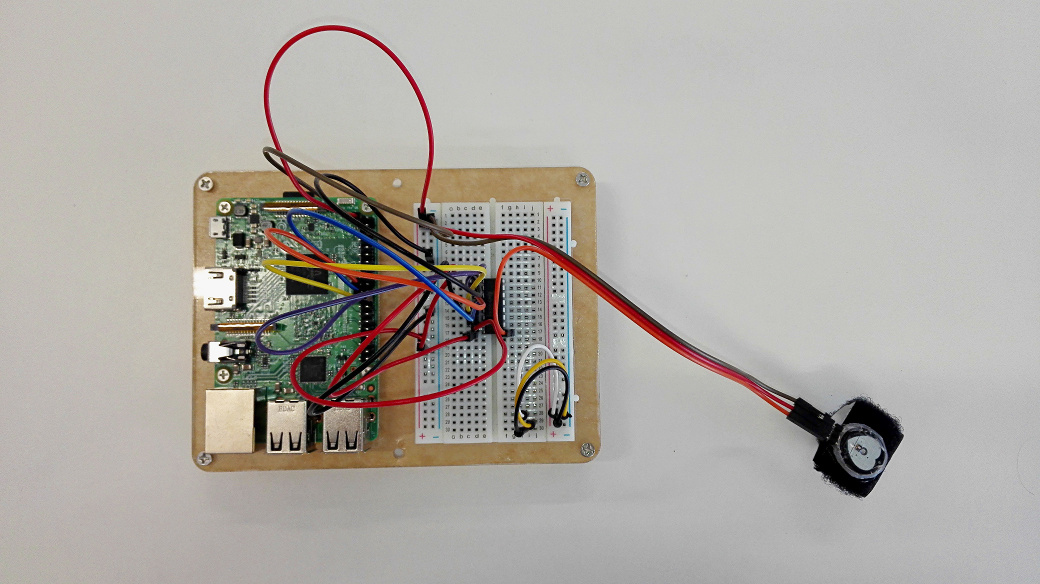
\includegraphics[width=10cm]{img/Chapter4/prototype1_edited.jpg}
\caption[Prototype setup]{\footnotesize{Prototype setup.}}
\end{figure}

\lipsum[14]

\subsection{Subsection 4.2}
\label{subsec:subsec4.2}

\begin{table}[H]
\centering
\caption[This is the caption]{ \footnotesize This is the other caption. Since the trial size of the experiments showed is one second, the number of \textit{Target} and \textit{Impostor} data corresponds to number of trials or seconds}
\label{tab:data_partition}
\footnotesize{
\begin{tabular}{@{}llcccc@{}}
\toprule
\textbf{Dataset}         & \multicolumn{1}{c}{\textbf{Label}} & \textbf{Train} & \textbf{Validation} & \textbf{Develop} & \textbf{Test} \\ \midrule
\midrule
\multirow{3}{*}{First} & Target   & $135$ & $45$  & $30$  & $30$  \\
                         & Impostor & $5,220$    & $1,740$ & $1,890$   & $2,880$    \\
\cmidrule(lr){3-5} \cmidrule(l){6-6}
                         & \#Subjects          & \multicolumn{3}{c}{$31$} & $12$ \\
\midrule
\multirow{3}{*}{Second}  & Target   & $144$ & $80$  & $48$  & $48$  \\
                         & Impostor & $2,014$    & $1,119$    & $1,343$    & $1,545$ \\
\cmidrule(lr){3-5} \cmidrule(l){6-6}
                         & \#Subjects   & \multicolumn{3}{c}{$15$} & $5$ \\ 
\bottomrule
\end{tabular}
}
\end{table}






%%%%%%%%%%%%%%%%%%%%%%%%%%%%%
%%% FINAL PART: SECTIONS %%%%
%%%%%%%%%%%%%%%%%%%%%%%%%%%%%

%%% 05-BUDGET %%%
\clearpage
\label{sec:budget}
\clearpage\section{Budget}
For the budget of this project, we should include:
\begin{itemize}
	\item{Single developer role. Total time of 600h at 12€/h.}
	\item{Double role for supervisor. Total time of 150h at 15€/h.}
	\item{Single laptop for development. Cost at 1000€.}
	\item{Server for development. Cost at 5000€.}
\end{itemize}
All sum ups a total of \textbf{17.700€} for the project.


%%% 06-CONCLUSIONS %%%
\clearpage
\label{sec:conclusions}
%\vspace*{2cm}
\section{Conclusions}
In this thesis we have achieved the following accomplishments:
\begin{itemize}
	\item{Improvement of the ``lxce'' command line tool in a more improved, tested version}
	\item{Added functionalities to the ``lxce-admin'' tool improving the management of the containers}
	\item{Complete build of an initial web application with a view for improvements and extensibility}
\end{itemize}

The main limitations were working and learning a new technology (``containerization'') not known at the beginning of the project, plus developing the set of tools in a programming language (javascript/typescript) without any previous experience. Also for development of the web application learning about React was needed.

Also, some systems administration research was needed for setting up the development environment.


%%% 07-FUTURE WORK %%%
\label{sec:futurework}
\section{Future work}
The next steps for this project would involve mainly:
\begin{itemize}
	\item{Integrate into the ``lxce'' command a new functionality involving web services in a way in we could define a web proxy and expose a service inside the container by a configuration file.}
	\item{Improve the web application integrating all the ``lxce'' commands along with extending the current API.}
\end{itemize}



%%%%%%%%%%%%%%%%%%%%%%%%%%%%
%%% EXTRA: SECTIONS %%%%%%%%
%%%%%%%%%%%%%%%%%%%%%%%%%%%%

%%% BIBLIOGRAPHY %%%

\newpage

\medskip

\bibliographystyle{unsrt}
\bibliography{bibliography.bib}
\nocite{*}     %% For listing all references

%%% EXTRA-ANNEX %%%
\clearpage
\newpage
\begin{appendices}
    %%%%%%%%%%%%%%%%%%%%%
%% APPENDIX-LXCE %%%%
%%%%%%%%%%%%%%%%%%%%%
\section{lxce}\label{annex:lxce}
For the commands that are available for our command, we have the following structure:
\begin{minted}[bgcolor=background]{text}
Usage: lxce [command] <options> <flags>

Commands:
  lxce alias       Manage containers aliases
  lxce completion  Output completions scripts
  lxce delete      Delete containers and configurations/folders related
  lxce init        Initialize lxce command
  lxce launch      Launch containers
  lxce list        List containers properties
  lxce pass        Compute password from containers
  lxce proxy       Delete and restart proxies 
  lxce rebase      Relaunch container with new base specified
  lxce show        Show containers configurations files
  lxce start       Start containers
  lxce stop        Stop containers
  lxce uninstall   Remove all configurations from the lxce command

Flags
      --version  Show version number        
  -h, --help     Show help                 
  -v, --verbose
\end{minted}

%%%%%%%%%%%%%%%%%%%%%%%%
%%% LIST OF COMMANDS %%%
\newpage
\textbf{lxce alias}
\begin{listing}[H]
\begin{minted}[bgcolor=background]{text}
Usage: lxce alias [command] <options> <flags>

Commands:
  lxce alias set    set container alias
  lxce alias unset  unset container alias
  lxce alias check  check container alias

Flags
      --version  Show version number                                   
  -h, --help     Show help                                             
  -v, --verbose
\end{minted}
\caption{lxce alias}
\label{listings: lxce alias}
\end{listing}

\textbf{lxce alias set}
\begin{listing}[H]
\begin{minted}[bgcolor=background]{text}
Usage: lxce alias set [options] <flags>

Options
  -d, --domain  container domain                             
  -n, --name    container name                               
  -a, --alias   new container alias                          

Flags
      --version  Show version number                                   
  -h, --help     Show help                                            
  -v, --verbose

Examples:
  lxce alias set -d google                Set alias alice to container 
  -n front -a alice                       front within google domain
\end{minted}
\caption{lxce alias set}
\label{listings: lxce alias set}
\end{listing}
\TODO{Change all descriptions to match [] or <>}

\newpage
\textbf{lxce alias unset}
\begin{listing}[H]
\begin{minted}[bgcolor=background]{text}
Usage: lxce alias unset [options] <flags>

Options
  -d, --domain  container domain                             
  -n, --name    container name                               
  -a, --alias   new container alias                          

Flags
      --version  Show version number                        
  -h, --help     Show help                                  
  -v, --verbose

Examples:
  lxce alias unset -d google -n front  Unset alias to container front 
                                       within google domain
  lxce alias unset -d google -a alice  Unset alias to container with 
                                       alice alias within google 
				       domain
\end{minted}
\caption{lxce alias unset}
\label{listings: lxce alias unset}
\end{listing}

\textbf{lxce alias check}
\begin{listing}[H]
\begin{minted}[bgcolor=background]{text}
Usage: lxce alias check [options] <flags>

Options
  -d, --domain  container domain                             
  -a, --alias   new container alias                          
  -f, --format  output format            ["plain", "json", "csv"]

Flags
      --version  Show version number                                   
  -h, --help     Show help                                             
  -v, --verbose

Examples:
  lxce alias check -d google -a alice  check alice alias existence 
                                       within google domain
\end{minted}
\caption{lxce alias check}
\label{listings: lxce alias check}
\end{listing}


\textbf{lxce delete}
\begin{listing}[H]
\begin{minted}[bgcolor=background]{text}
Usage: lxce delete <options> <flags>

Options
  -g, --global  apply to all containers                         
  -d, --domain  domain name for a group of containers            
  -n, --name    container name                                   
  -a, --alias   container alias                                 
  -y, --yes     yes to questions                                

Flags
      --version  Show version number                            
  -h, --help     Show help                                      
  -v, --verbose

Examples:
  lxce delete --global                   Deletes all containers and
                                         configurations related
  lxce delete -d google                  Deletes all containers within 
                                         google domain
  lxce delete -d google -n still-yellow  Deletes container referenced 
                                         by name
  lxce delete -d google -a alice         Deletes container referenced
                                         by alias
\end{minted}
\caption{lxce delete}
\label{listings: lxce delete}
\end{listing}

\textbf{lxce init}
\begin{listing}[H]
\begin{minted}[bgcolor=background]{text}
Usage: lxce init <flags>

Flags
      --version  Show version number                            
  -h, --help     Show help                                      
  -v, --verbose
\end{minted}
\caption{lxce init}
\label{listings: lxce init}
\end{listing}

\newpage
\textbf{lxce launch}
\begin{listing}[H]
\begin{minted}[bgcolor=background]{text}
Usage: lxce launch <options> <flags>

Options
  -d, --domain   domain for the container/containers         
  -r, --range    range of container (ex: -r 5)             
  -n, --names    names/name of the containers/container                  
  -a, --aliases  aliases/alias of the containers/container               

Flags
      --version  Show version number                                   
  -h, --help     Show help                                             
  -v, --verbose

Examples:
  lxce launch -d google                     Launch one container within 
                                            google with a random name
  lxce launch -d google -r 3                Launch three containers 
                                            within google with 
					    random names
  lxce launch -d google -r 3 -n back front  Launch three containers 
  base                                      within google with 
                                            specified names
  lxce launch -d google -r 3 -n back front  Launch three containers with 
  base -a alice bob eve                     name and alias
                                            specified
  lxce launch -d google -r 3 -a alice bob   Launch three containers 
  eve                                       with random names and 
                                            alias specified
\end{minted}
\caption{lxce launch}
\label{listings: lxce launch}
\end{listing}

\newpage
\textbf{lxce list}
\begin{listing}[H]
\begin{minted}[bgcolor=background]{text}
Usage: lxce <options> <flags>

Format options
==============
-n: "name"
-a: "alias"
-u: "user"
-b: "base"
-r: "ram (MB)"
-p: "ports"
-4: "ipv4"
-6: "ipv6"
-s: "status"
-d: "domain"
-c: "cpu usage (s)"

Options
  -c, --columns  Values to show                                         
  -f, --format   Output format                                          

Flags
      --version  Show version number                                   
  -h, --help     Show help                                             
  -v, --verbose

Examples:
  lxce list -c naubr
  lxce list -f json
\end{minted}
\caption{lxce list}
\label{listings: lxce list}
\end{listing}

\newpage
\textbf{lxce pass}
\begin{listing}[H]
\begin{minted}[bgcolor=background]{text}
Usage: lxce pass <options> <flags>

Options
  -g, --global  Apply to all containers                               
  -d, --domain  Domain name for a group of containers                 
  -n, --name    Container name                                        
  -a, --alias   Container alias                                       
  -p, --plain   plain output                                          

Flags
      --version  Show version number                                  
  -h, --help     Show help                                            
  -v, --verbose

Examples:
  lxce pass --global            Compute all container passwords
  lxce pass --domain google     Compute all domain passwords
  lxce pass -d google -n front  Compute container name password
  lxce pass -d google -a alice  Compute container alias password

\end{minted}
\caption{lxce pass}
\label{listings: lxce pass}
\end{listing}

\newpage
\textbf{lxce proxy}
\begin{listing}[H]
\begin{minted}[bgcolor=background]{text}
Usage: lxce proxy <options> <flags>

Options
  -g, --global  Apply to all containers                                
  -d, --domain  Domain name for a group of containers                  
  -n, --name    Container name                                         
  -a, --alias   Container alias                                        

Flags
      --version  Show version number                                   
  -h, --help     Show help                                             
  -v, --verbose

Examples:
  lxce proxy --global            Restart all containers proxies based 
                                 on their configuration files
  lxce proxy -d google           Restart all domain containers proxies 
                                 based on their configuration files
  lxce proxy -d google -n front  Restart container proxies
  lxce proxy -d google -a alice  Restart container proxies
\end{minted}
\caption{lxce proxy}
\label{listings: lxce proxy}
\end{listing}

\newpage
\textbf{lxce rebase}
\begin{listing}[H]
\begin{minted}[bgcolor=background]{text}
Usage: lxce rebase <options> <flags>

Options
  -g, --global  Applied to all containers                              
  -d, --domain  Domain name for a group of containers                  
  -n, --name    Container name                                         
  -a, --alias   Container alias                                        
  -b, --base    Container base                               

Flags
      --version  Show version number                                   
  -h, --help     Show help                                             
  -v, --verbose

Examples:
  lxce rebase --global                   Applies new base to existing 
                                         containers and future ones
  lxce rebase -d google                  Applies new base to all
                                         containers withing 
                                         google domain
  lxce rebase -d google -n still-yellow  Applies new base to container 
  lxce rebase -d google -a alice         Applies new base to container 
\end{minted}
\caption{lxce rebase}
\label{listings: lxce rebase}
\end{listing}

\newpage
\textbf{lxce show}
\begin{listing}[H]
\begin{minted}[bgcolor=background]{text}
Usage: lxce show <options> <flags>

Options
  -g, --global  Apply to all containers                                
  -d, --domain  Domain name for a group of containers                  
  -n, --name    Container name                                         
  -a, --alias   Container alias                                        
  -e, --extra   Show extra information                

Flags
      --version  Show version number                                   
  -h, --help     Show help                                             
  -v, --verbose

Examples:
  lxce show --global                   Show all containers configurations
  lxce show -d google                  Show all containers configurations 
                                       within domain
  lxce show -d google -n still-yellow  Show container configurations 
                                       defined by name
  lxce show -d google -a alice         Stop container configuration 
                                       defined by alias
\end{minted}
\caption{lxce show}
\label{listings: lxce show}
\end{listing}

\newpage
\textbf{lxce start}
\begin{listing}[H]
\begin{minted}[bgcolor=background]{text}
Usage: lxce start <options> <flags>

Options
  -g, --global  Apply to all containers                                
  -d, --domain  Domain name for a group of containers                  
  -n, --name    Container name                                         
  -a, --alias   Container alias                                        

Flags
      --version  Show version number                                   
  -h, --help     Show help                                             
  -v, --verbose

Examples:
  lxce start --global                   Start all containers
  lxce start -d google                  Start all container within domain
  lxce start -d google -n still-yellow  Start container defined by name
  lxce start -d google -a alice         Start container defined by alias
\end{minted}
\caption{lxce start}
\label{listings: lxce start}
\end{listing}

\newpage
\textbf{lxce stop}
\begin{listing}[H]
\begin{minted}[bgcolor=background]{text}
Usage: lxce stop <options> <flags>

Options
  -g, --global  Apply to all containers                                
  -d, --domain  Domain name for a group of containers                  
  -n, --name    Container name                                         
  -a, --alias   Container alias                                        

Flags
      --version  Show version number                                   
  -h, --help     Show help                                             
  -v, --verbose

Examples:
  lxce stop --global                   Stop all containers
  lxce stop -d google                  Stop all container within domain
  lxce stop -d google -n still-yellow  Stop container defined by name
  lxce stop -d google -a alice         Stop container defined by alias
\end{minted}
\caption{lxce stop}
\label{listings: lxce stop}
\end{listing}

\textbf{lxce uninstall}
\begin{listing}[H]
\begin{minted}[bgcolor=background]{text}
lxce uninstall <options> <flags>

Options
  -y, --yes                                                            

Flags
      --version  Show version number                                   
  -h, --help     Show help                                             
  -v, --verbose
\end{minted}
\caption{lxce uninstall}
\label{listings: lxce uninstall}
\end{listing}
%% END OF COMMANDS %%%%%
%%%%%%%%%%%%%%%%%%%%%%%%

    %%%%%%%%%%%%%%%%%%%%%%%%%%%
%% APPENDIX-LXCE-ADMIN %%%%
%%%%%%%%%%%%%%%%%%%%%%%%%%%
\newpage\section{lxce-admin}\label{annex:lxce-admin}

%%%%%%%%%%%%%%%%%%%%%%%%
%%% LIST OF COMMANDS %%%
\textbf{lxce-admin config}
\begin{minted}[bgcolor=background]{text}
Usage: lxce-admin [command] <flags>

Commands:
  lxce-admin config add     Add host and sync files
  lxce-admin config list    List configured hosts
  lxce-admin config remove  Remove host and associated files
  lxce-admin config update  Update host associated files

Flags
      --version  Show version number                                   
  -h, --help     Show help                                             
  -v, --verbose
\end{minted}

\textbf{lxce-admin config add}
\begin{minted}[bgcolor=background]{text}
Usage: lxce-admin config add <options> <flags>

Options
      --dry-run                                                        

Flags
      --version  Show version number                                   
  -h, --help     Show help                                             
  -v, --verbose
\end{minted}

\textbf{lxce-admin config list}
\begin{minted}[bgcolor=background]{text}
Usage: lxce-admin config list

Flags
      --version  Show version number                                   
  -h, --help     Show help                                             
  -v, --verbose
\end{minted}

\textbf{lxce-admin config remove}
\begin{minted}[bgcolor=background]{text}
Usage: lxce-admin config remove <options> <flags>

Options
      --host     configured host                             
      --dry-run                                              

Flags
      --version  Show version number                                   
  -h, --help     Show help                                             
  -v, --verbose
\end{minted}

\textbf{lxce-admin config update}
\begin{minted}[bgcolor=background]{text}
Usage: lxce-admin config update <options> <flags>

Flags
      --version  Show version number                                   
  -h, --help     Show help                                             
  -v, --verbose
\end{minted}

\newpage
\textbf{lxce-admin pass}
\begin{minted}[bgcolor=background]{text}
Usage: lxce-admin pass <options> <flags>

Options
      --host    configured host                              
  -d, --domain  container domain                             
  -n, --name    container name                               
  -a, --alias   container alias                              

Flags
      --version  Show version number                        
  -h, --help     Show help                                  
  -v, --verbose
\end{minted}

\textbf{lxce-admin remmina}
\begin{minted}[bgcolor=background]{text}
Usage: lxce-admin remmina <options> <flags>

Options
      --host    configured host                              
  -d, --domain  container domain                             
  -n, --name    container name                               
  -a, --alias   container alias                              

Flags
      --version  Show version number                        
  -h, --help     Show help                                  
  -v, --verbose
\end{minted}

\newpage
\textbf{lxce-admin vnc}
\begin{minted}[bgcolor=background]{text}
Usage: lxce-admin vnc <options> <flags>

Options
      --host     configured host                             
  -d, --domain   container domain                            
  -n, --name     container name                              
  -a, --alias    container alias                             
      --scale    scale vnc viewer                            
      --dry-run                                              

Flags
      --version  Show version number                        
  -h, --help     Show help                                  
  -v, --verbose
\end{minted}
%%% END OF COMMANDS %%%
%%%%%%%%%%%%%%%%%%%%%%%%

    %%%%%%%%%%%%%%%%%%%%%
%% APPENDIX-LXCE-CONF %%%%
%%%%%%%%%%%%%%%%%%%%%
\newpage\newpage\section{Configuration files}

\begin{listing}[H]
\begin{minted}[bgcolor=background]{text}
/etc/lxce 
|--- container.conf.d 			
|   |--- default 			
|   |   '--- voiceless-blue
|   '--- derecho 			
|       '--- relieved-beige
|--- container_default.conf 		
|--- lxce.conf 			
|--- remmina 		
|   |--- default 
|   |   '--- oscar-vm.default.voiceless-blue.remmina
|   '--- derecho 
|       '--- oscar-vm.derecho.relieved-beige.remmina
'--- ssh 	
    |--- default 
    |   '--- voiceless-blue.conf
    '--- derecho
        '--- relieved-beige.conf
\end{minted}
\caption{lxce directory structure}
\label{listings: lxce directory structure /etc/lxce}
\end{listing}

In this way we are able to manage the container configurations from our command line and update/delete files based on the state of the command.

Where the configurations files content is the following:
\begin{itemize}
%%%%%%%%%%
%% ITEM %%
%%%%%%%%%%
\newpage
\item{\textbf{container-default.conf}

This file acts as a template for every container to be created.
\begin{listing}[H]
\begin{minted}[bgcolor=background]{json}
{
  "name": "",                           
  "alias": "",                          
  "user": "",
  "id_domain": 0,
  "id_container": 0,

  "domain": "default",                 
  "base": "ubuntu:20.04",             
  "userData": "/datasdd",            

  "proxies": [                      
    {
      "name": "ssh",
      "type": "tcp",
      "listen": "0.0.0.0",
      "port": 22
    },
    {
      "name": "test",
      "type": "tcp",
      "listen": "0.0.0.0",
      "port": 3000
    }
  ],
}
\end{minted}
\caption{/etc/lxce/container-default.conf}
\label{listings: /etc/lxce/container-default.conf}
\end{listing}
\TODO{Think the convention for the name of the figures and the descriptions of the listings}
}
%%%%%%%%%%
%% ITEM %%
%%%%%%%%%%
\newpage
\item{\textbf{lxce.conf}

This file specifies different parameters of the host where the command is installed, such as:
\begin{itemize}
	\item{SSH IP}
	\item{Hostname}
	\item{Local VNC server configuration}
	\item{Seed used for generating passwords}
	\item{List of container domains currently in the host}
	\item{List of locations available for the shared containers folders location}
\end{itemize}
\begin{listing}[H]
\begin{minted}[bgcolor=background]{json}
{
  "hypervisor": {
    "SSH_hostname": "localhost",
    "SSH_suffix": "oscar-vm",
    "VNC_server": "localhost",
    "VNC_port": 5901
  },
  "seed": "4b5a003f0e1715df",
  "domains": [
    {
      "id": 0,
      "name": "default"
    },
    {
      "id": 1,
      "name": "derecho"
    }
  ],
  "locations": [
    "/datasdd"
  ]
}
\end{minted}
\caption{lxce.conf}
\label{listings: /etc/lxce/lxce.conf}
\TODO{explain all the parameters}
\end{listing}
}
%%%%%%%%%%
%% ITEM %%
%%%%%%%%%%
\newpage
\item{\textbf{container configuration file}

This files list the configured parameters for each container and the ids that uniquelly identifies it
\begin{listing}[H]
\begin{minted}[bgcolor=background]{json}
{
  "name": "voiceless-blue",
  "alias": "",
  "user": "ubuntu",
  "id_domain": 0,
  "id_container": 0,
  "domain": "default",
  "base": "ubuntu:20.04",
  "userData": "/datasdd",
  "proxies": [
    {
      "name": "ssh",
      "type": "tcp",
      "listen": "0.0.0.0",
      "port": 22
    },
    {
      "name": "test",
      "type": "tcp",
      "listen": "0.0.0.0",
      "port": 3000
    }
  ],
}
\end{minted}
\caption{container configuration file}
\label{listings: /etc/lxce/container.conf.d/default/voiceless-blue}
\end{listing}
}
%%%%%%%%%%
%% ITEM %%
%%%%%%%%%%
\clearpage
\item{\textbf{VNC configuration}
\begin{listing}[H]
\begin{minted}[bgcolor=background]{text}
[remmina]
ssh_tunnel_privatekey=
name=oscar-vm.default.voiceless-blue          # Container name
ssh_tunnel_passphrase=
password=.                                    # For saving VNC password
...
server=localhost:5901                         # VNC server
disablepasswordstoring=0
ssh_tunnel_username=ubuntu
disableclipboard=0
window_maximize=1
ssh_tunnel_password=.                         # For saving ssh password
enable-autostart=0
proxy=
ssh_tunnel_server=localhost:10000             # Container SSH Port
ssh_tunnel_auth=0
group=oscar-vm.upc.edu                        
...
protocol=VNC
username=ubuntu                               # VNC username
showcursor=0
colordepth=32

\end{minted}
\caption{REMMINA configuration file}
\label{listing: /etc/lxce/remmina/default/oscar-vm.default.voiceless-blue.remmina}
\end{listing}
}
%%%%%%%%%%
%% ITEM %%
%%%%%%%%%%
\item{\textbf{SSH configuration}
\begin{listing}[H]
\begin{minted}[bgcolor=background]{text}
Host oscar-vm.default.voiceless-blue
   Hostname localhost
   User ubuntu
   Port 10000
   TCPKeepAlive yes
   ServerAliveInterval 300
\end{minted}
\caption{ssh configuration file}
\label{listings: /etc/lxce/ssh/default/voiceless-blue.conf}
\end{listing}
}
\end{itemize}

\end{appendices}
\end{document}
